\documentclass[12pt]{aghdpl}
% \documentclass[en,11pt]{aghdpl}  % praca w języku angielskim

% Lista wszystkich języków stanowiących języki pozycji bibliograficznych użytych w pracy.
% (Zgodnie z zasadami tworzenia bibliografii każda pozycja powinna zostać utworzona zgodnie z zasadami języka, w którym dana publikacja została napisana.)
\usepackage[english,polish]{babel}

% Użyj polskiego łamania wyrazów (zamiast domyślnego angielskiego).
\usepackage{polski}

\usepackage[utf8]{inputenc}

% dodatkowe pakiety

\usepackage{mathtools}
\usepackage{amsfonts}
\usepackage{amsmath}
\usepackage{amsthm}
\usepackage[percent]{overpic}

% --- < bibliografia > ---

\usepackage[
style=numeric,
sorting=none,
%
% Zastosuj styl wpisu bibliograficznego właściwy językowi publikacji.
language=autobib,
autolang=other,
% Zapisuj datę dostępu do strony WWW w formacie RRRR-MM-DD.
urldate=iso8601,
% Nie dodawaj numerów stron, na których występuje cytowanie.
backref=false,
% Podawaj ISBN.
isbn=true,
% Nie podawaj URL-i, o ile nie jest to konieczne.
url=false,
%
% Ustawienia związane z polskimi normami dla bibliografii.
maxbibnames=3,
% Jeżeli używamy BibTeXa:
backend=bibtex
]{biblatex}

\usepackage{csquotes}
% Ponieważ `csquotes` nie posiada polskiego stylu, można skorzystać z mocno zbliżonego stylu chorwackiego.
\DeclareQuoteAlias{croatian}{polish}

\addbibresource{bibliografia.bib}

% Nie wyświetlaj wybranych pól.
%\AtEveryBibitem{\clearfield{note}}


% ------------------------
% --- < listingi > ---

% Użyj czcionki kroju Courier.
\usepackage{times}

\usepackage{listings}
\lstloadlanguages{TeX}

\lstset{
	literate={ą}{{\k{a}}}1
           {ć}{{\'c}}1
           {ę}{{\k{e}}}1
           {ó}{{\'o}}1
           {ń}{{\'n}}1
           {ł}{{\l{}}}1
           {ś}{{\'s}}1
           {ź}{{\'z}}1
           {ż}{{\.z}}1
           {Ą}{{\k{A}}}1
           {Ć}{{\'C}}1
           {Ę}{{\k{E}}}1
           {Ó}{{\'O}}1
           {Ń}{{\'N}}1
           {Ł}{{\L{}}}1
           {Ś}{{\'S}}1
           {Ź}{{\'Z}}1
           {Ż}{{\.Z}}1,
	basicstyle=\footnotesize\ttfamily,
}

% ------------------------

\AtBeginDocument{
	\renewcommand{\tablename}{Tabela}
	\renewcommand{\figurename}{Rys.}
}

% ------------------------
% --- < tabele > ---

\usepackage{array}
\usepackage{tabularx}
\usepackage{multirow}
\usepackage{booktabs}
\usepackage{makecell}
\usepackage[flushleft]{threeparttable}
\usepackage{graphicx}
\usepackage[]{algorithm2e}
\usepackage{float}
\graphicspath{ {images/} }
\usepackage{etoolbox}
\makeatletter
\patchcmd{\chapter}{\if@openright\cleardoublepage\else\clearpage\fi}{}{}{}
\makeatother


% defines the X column to use m (\parbox[c]) instead of p (`parbox[t]`)
\newcolumntype{C}[1]{>{\hsize=#1\hsize\centering\arraybackslash}X}


%---------------------------------------------------------------------------

\author{Jakub Tańcula, Wiktor Wąsowicz}
\shortauthor{}

%\titlePL{Przygotowanie bardzo długiej i pasjonującej pracy dyplomowej w~systemie~\LaTeX}
%\titleEN{Preparation of a very long and fascinating bachelor or master thesis in \LaTeX}
\course{Laboratorium Problemowe}
\titlePL{Serwomechanizm}
\titleEN{}


\shorttitlePL{} % skrócona wersja tytułu jeśli jest bardzo długi
%\shorttitleEN{Preparation of a long and fascinating thesis in \LaTeX}

%\thesistype{Laboratorium problemowe - sprawozdanie}
%\thesistype{Master of Science Thesis}

\supervisor{dr hab. inż. Adam Piłat}
%\supervisor{Marcin Szpyrka PhD, DSc}

\degreeprogramme{Automatyka i Robotyka}
%\degreeprogramme{Computer Science}

\date{2017}

\department{Katedra Automatyki i Inżynierii Biomedycznej}
%\department{Department of Applied Computer Science}

\faculty{Wydział Elektrotechniki, Automatyki,\protect\\[-1mm] Informatyki i Inżynierii Biomedycznej}
%\faculty{Faculty of Electrical Engineering, Automatics, Computer Science and Biomedical Engineering}

\acknowledgements{}


\setlength{\cftsecnumwidth}{10mm}

%---------------------------------------------------------------------------
\setcounter{secnumdepth}{4}
\brokenpenalty=10000\relax


\begin{document}

\titlepages


% Ponowne zdefiniowanie stylu `plain`, aby usunąć numer strony z pierwszej strony spisu treści i poszczególnych rozdziałów.
\fancypagestyle{plain}
{
	% Usuń nagłówek i stopkę
	\fancyhf{}
	% Usuń linie.
	\renewcommand{\headrulewidth}{0pt}
	\renewcommand{\footrulewidth}{0pt}
}


\setcounter{tocdepth}{2}
\tableofcontents
\clearpage



%\include{tests}


\chapter{Wstęp}
\label{cha:Wstep}
%---------------------------------------------------------------------------

W ramach zajęć laboratorium problemowego zostało postawione przed nami zadanie stworzenia regulatorów serwomechanizmu napędzanego przez silnik prądu stałego pozwalający na sterowanie położeniem wału serwomechnizmu. % TODO CZY TO WAŁ
Schemat obiektu został przedstawiony na rysunku \ref{fig:Schemat}. W trakcie prac nad regulatorem korzystano z komputera, pakietu Matlab/simulink/
%\begin{figure}[h]
%	% TODO UWAGA ZROBIC WLASNY RYSUNEK !!!!!!!!
%%	\includegraphics[width=1\textwidth]{wstep/schemat}
%	\centering
%	\caption{Schemat stanowiska laboratoryjnego.}
%	\label{fig:Schemat}
%\end{figure}











\chapter{Identyfikacja}
\label{cha:Identyfikacja}
%---------------------------------------------------------------------------

\section{Model matematyczny}
\label{sec:model_mat}
W celu wyznaczenia modelu matematycznego omawianego obiektu posłużono się rówaniami elektrycznym \ref{eq:elekt} oraz mechanicznym \ref{eq:mechaniczne} silnika
\begin{figure}[H]

	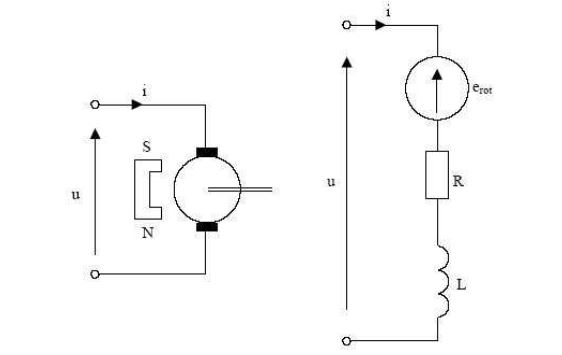
\includegraphics[width=0.5\textwidth]{identyfikacja/model_silnika}
	\centering
	\caption{Model silnika prądu stałego.}
	\label{fig:Schemat}
\end{figure}



\begin{equation}
\label{eq:elekt}
u(t)= R \cdot i(t) + L \frac{d}{dt}i(t) + e_{rot}
\end{equation}

\begin{equation}
\label{eq:mechaniczne}
J \cdot \frac{d}{dt} \omega(t) = K_{E} \cdot \phi \cdot i(t)
\end{equation}
gdzie:
\newline $e_{rot} = k_{E} \cdot \phi \cdot \omega(t)$

gdzie:

R - rezystancja uzwojeń twornika,
L - indukcyjność uzwojeń twornika,
$e_{rot}$ - siła elektromotoryczna,
J - moment bezwłądności silnika,
$\phi$ -strumień wzbuczenia od magnesów trwałych
$k_E$ - wsppółczynnik proporcjonalności wiążący napięcie rotacji z prędkością kątową oraz moment elektromagnetyczny z prądem twornika% TODO co to jest ?
 
%\begin{equation}
%\label{eq:e_rot}
%e_{rot} = k_{E} \cdot \phi \cdot \omega(t)
%\end{equation}

Skąd otrzymano układ równań silnika w postaci operatorowej postaci \ref{eq:oper}

\begin{equation}
\label{eq:oper}
\left\{ \begin{array}{ll}
U(s)  = R \cdot I(s) + L \cdot I(s) \cdot s + k_{E} \cdot \phi \cdot \Omega(s)\\
J \cdot \Omega(s) \cdot s  = K_{E} \cdot \phi \cdot I(s)
\end{array} \right.
\end{equation}

 Skąd po przekształceniach otrzymano wzór na transmitancję układu \ref{eq:transmitancja_pred}
\begin{equation}
\label{eq:transmitancja_pred}
G(s) = \frac{\Omega(s)}{U(s)} = \frac{K}{T \cdot s + 1}
\end{equation}

Jest to transmitancja obiektu pierwszego rzędu opisującą zależność obrotów silnika od napięcia wejściowgo, natomiast transmitancja \ref{eq:transmitancja_kat}:
\begin{equation}
\label{eq:transmitancja_kat}
G(s) = \frac{\alpha(s)}{U(s)} = \frac{ K}{s \cdot (T \cdot s + 1)}
\end{equation}
opisuje zależność kąta wału silnika od napięcia wejściowego. Jest to transmitancja obiektu inercyjnego z członem całkującym

\section{Martwa strefa}
W trakcie badań nad systemem zauważono, że występuje w nim zjawisko martwej strefy. Zostało ono przedstawione na rysunku \ref{fig:martwa_sterfa}
\begin{figure}[H]
	
	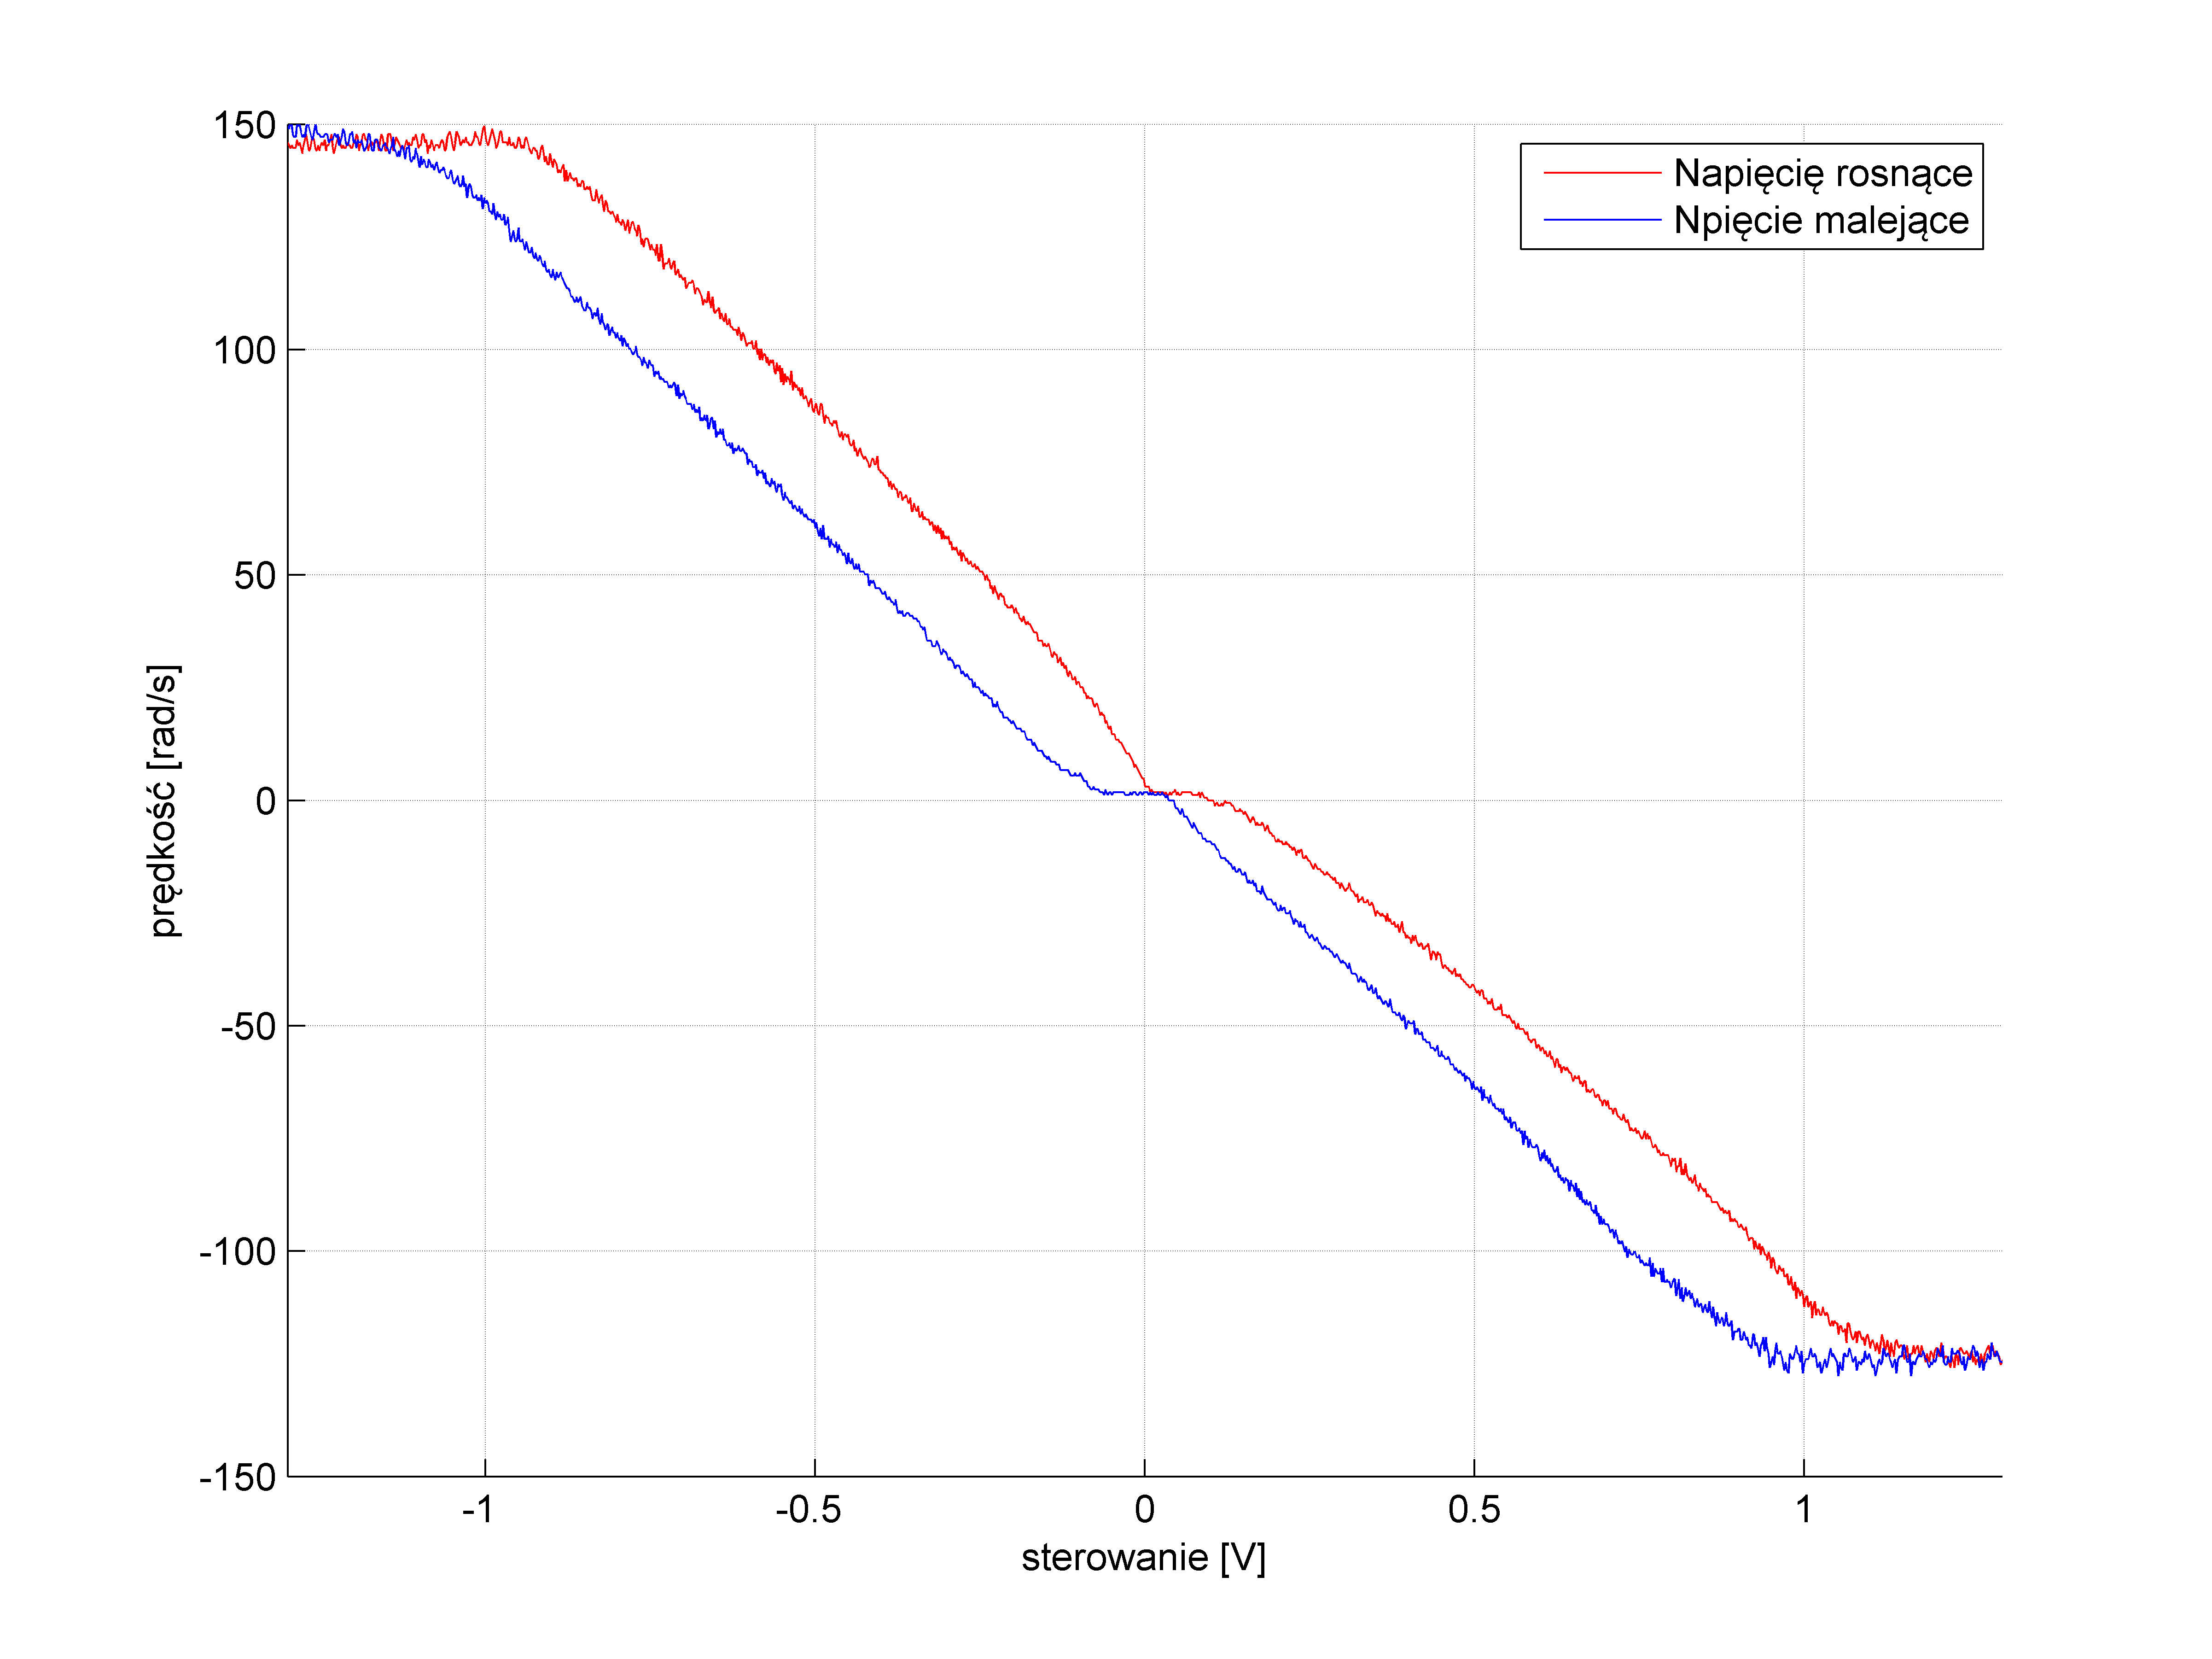
\includegraphics[width=0.7\textwidth]{identyfikacja/martwa_strefa}
	\centering
	\caption{Martwa strefa silnika.}
	\label{fig:martwa_sterfa}
\end{figure}

Na podstawie powyższego rysunku można stwierdzić iż silnik posiada niesymetryczną martwą strefę. Dla napięcia rosnącego źle źle źle źle!!!! w modelu nie uwzględniamy napięcia rosnącego lub malejącego tylko ujemne i dodatnie!!!! kurwa
\section{Modele}
\subsection*{Model z pojedynczej transmitancji}
\subsection*{Model z podwójnej transmitancji}

\chapter{Regulator PID}
\label{cha:PID}


% itd.
% \appendix
% \include{dodatekA}
% \include{dodatekB}
% itd.




\end{document}
